\documentclass[aspectratio=169, 10pt]{beamer}

% Thème
\usetheme{Madrid}
\usecolortheme{beaver}
\setbeamertemplate{navigation symbols}{}
\setbeamertemplate{footline}[frame number]

% Packages
\usepackage{tikz}
\usetikzlibrary{shapes, arrows, positioning, fit, backgrounds, patterns, matrix, calc, shapes.geometric}
\usepackage{pgfplots}
\pgfplotsset{compat=1.17}
\usepackage{listings}
\usepackage{xcolor}
\usepackage{booktabs}

% Couleurs personnalisées
\definecolor{codebg}{rgb}{0.95,0.95,0.95}
\definecolor{cudagreen}{RGB}{118,185,0}
\definecolor{memblue}{RGB}{100,149,237}
\definecolor{coreorange}{RGB}{255,140,0}

% Configuration Listings
\lstset{
    backgroundcolor=\color{codebg},
    basicstyle=\ttfamily\scriptsize,
    keywordstyle=\color{blue}\bfseries,
    commentstyle=\color{green!60!black},
    stringstyle=\color{red},
    frame=single,
    breaklines=true,
    language=C++
}

\title{Optimisation du Game of Life sur GPU}
\subtitle{De l'implémentation naïve au Bit-Packing}
\author{A5 TP Conway}
\date{NVIDIA RTX 3080 --- Grille 32k $\times$ 32k}

\begin{document}

% -----------------------------------------------------------------------------
% TITRE
% -----------------------------------------------------------------------------
\begin{frame}
    \titlepage\centering
    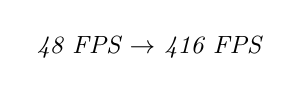
\begin{tikzpicture}
        \node[font=\small\itshape] {48 FPS $\to$ 416 FPS};
    \end{tikzpicture}
\end{frame}

% -----------------------------------------------------------------------------
% PARTIE 1: NOIF-CHAR
% -----------------------------------------------------------------------------
\section{Version Naïve: noif-char}

\begin{frame}{Version 1: noif-char (Naïve)}
    \begin{columns}
        \column{0.4\textwidth}

        \textbf{Taille grille:}
        $32768 \times 32768$ octets \\
        $\approx 1$ Go de RAM

        \vspace{0.5cm}
        \textbf{FPS:} 48.69 \\
        Type des données: \texttt{char} (1 octet = 1 cellule)\\
        Pas de shared memory

        \vspace{0.5cm}
        \textbf{Taille bloc:} 32$\times$32 threads (calculent 32$\times$32 cellules)
        

        
        \column{0.6\textwidth}
        \begin{center}
        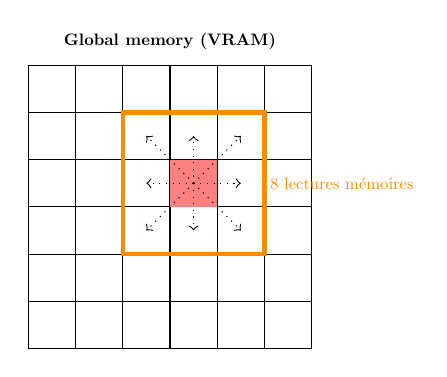
\begin{tikzpicture}[scale=0.6, transform shape]
            % Global Memory Grid
            \draw[fill=memblue!20] (0,0) grid (6,6);
            \node at (3,6.5) {\textbf{Global memory (VRAM)}};
            
            % Thread accessing neighbors
            \fill[red!50] (3,3) rectangle (4,4) node[midway, black] {};
            \draw[ultra thick, coreorange] (2,2) rectangle (5,5);
            \node[coreorange, right] at (5,3.5) {8 lectures mémoires};
            
            % Arrows representing access
            \foreach \xidx in {2,3,4} {
                \foreach \yidx in {2,3,4} {
                     \ifnum\xidx=3 
                        \ifnum\yidx=3 \else \draw[->, dotted] (3.5,3.5) -- (\xidx+0.5,\yidx+0.5); \fi 
                     \else 
                        \draw[->, dotted] (3.5,3.5) -- (\xidx+0.5,\yidx+0.5); 
                     \fi
                }
            }
        \end{tikzpicture}
        \end{center}
    \end{columns}
\end{frame}

\begin{frame}[fragile]{Logique ``branchless'' (noif)}
    \begin{lstlisting}
// On compte les voisins vivants
int neighbors = 0;
for (int dy = -1; dy < 2; dy++) {
    for (int dx = -1; dx < 2; dx++) {
        if (x + dx >= 0 && x + dx < width && y + dy >= 0 && y + dy < height && (dy != 0 || dx != 0)) {
        neighbors += grid[idx + dx + dy * width];
        }
    }
}

// Calcul conditionnel sans 'if'
int alive = (neighbors == 3) | (grid[y * width + x] == 1 && neighbors == 2);
new_grid[idx] = alive;
    \end{lstlisting}
    
    \vspace{0.5cm}
    \centering
    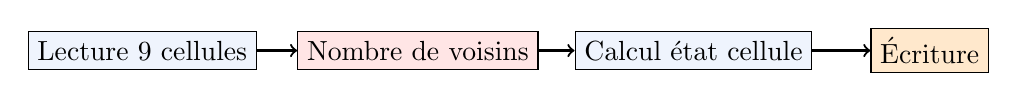
\begin{tikzpicture}
        \node[draw, fill=memblue!10, minimum width=2cm] (read) {Lecture 9 cellules};
        \node[draw, fill=red!10, right of=read, xshift=2.5cm] (nei) {Nombre de voisins};
        \node[draw, fill=memblue!10, right of=nei, xshift=2.5cm] (alu) {Calcul état cellule};
        \node[draw, fill=coreorange!20, right of=alu, xshift=2cm] (write) {Écriture};
        
        \draw[->, thick] (read) -- (nei);
        \draw[->, thick] (nei) -- (alu);
        \draw[->, thick] (alu) -- (write);
    \end{tikzpicture}
\end{frame}

% -----------------------------------------------------------------------------
% PARTIE 2: LOOKUP4X4
% -----------------------------------------------------------------------------

\begin{frame}{Version 2: Lookup table \texorpdfstring{4$\times$4}{4$\times$4}}
    \begin{columns}
        \column{0.4\textwidth}
        \textbf{Performance:}
        \begin{itemize}
            \item \textbf{FPS:} 112.76 ($\times 2.3$)
            \item \textbf{Stratégie:} Pré-calcul (LUT)
            \item \textbf{Mémoire:} Utilisation de la \textbf{shared memory}
        \end{itemize}
        
        \vspace{0.2cm}
        \textbf{Concept:}
        Réduire les calculs (comptage voisins) par une simple lecture tableau.
        
        \column{0.6\textwidth}
        \centering
        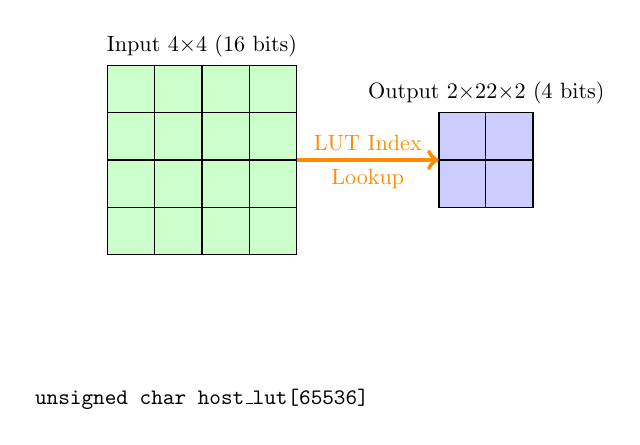
\begin{tikzpicture}[scale=0.8, transform shape]
            % LUT Idea
            \node[draw, fill=green!20, minimum width=3cm, minimum height=3cm, label=above:Input 4$\times$4 (16 bits)] (input) {};
            \draw[step=0.75] (-1.5,-1.5) grid (1.5,1.5);
            
            \node[draw, fill=blue!20, right=2.25cm of input, minimum width=1.5cm, minimum height=1.5cm, label=above:Output \texorpdfstring{2$\times$2}{2$\times$2} (4 bits)] (output) {};
            \draw[step=0.75] (3.74,-0.75) grid (5.25,0.75);
            
            \draw[->, ultra thick, coreorange] (input) -- node[above] {LUT Index} node[below] {Lookup} (output);
            
            \node[below=2cm of input] {\texttt{unsigned char host\_lut[65536]}};
        \end{tikzpicture}
    \end{columns}
\end{frame}

\begin{frame}[fragile]{Construction de l'index LUT}
    \begin{columns}
        \column{0.5\textwidth}
        \begin{lstlisting}
// Construction de l'index 16-bits
uint16_t state_idx = 0;
#pragma unroll
for (int r = 0; r < 4; r++) {
  #pragma unroll
  for (int c = 0; c < 4; c++) {
    if (tile[tile_r + r][tile_c + c]) {
       state_idx |= (1 << (r * 4 + c));
    }
  }
}
unsigned char res = lut[state_idx];
        \end{lstlisting}
        \column{0.5\textwidth}
        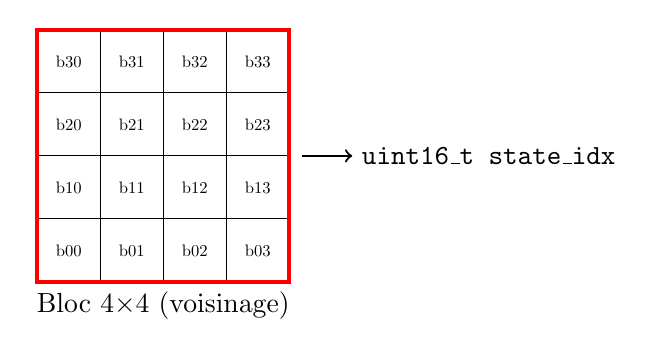
\begin{tikzpicture}[scale=0.8]
            % Visualizing the unroll
            \foreach \y in {0,1,2,3} {
                \foreach \x in {0,1,2,3} {
                    \draw (\x, \y) rectangle (\x+1, \y+1);
                    \node[scale=0.6] at (\x+0.5, \y+0.5) {b\y\x};
                }
            }
            \draw[ultra thick, red] (0,0) rectangle (4,4);
            \node[below] at (2,0) {Bloc 4$\times$4 (voisinage)};
            
            \draw[->, thick] (4.2, 2) -- (5, 2);
            \node[right] at (5, 2) {\texttt{uint16\_t state\_idx}};
        \end{tikzpicture}
    \end{columns}
\end{frame}

\begin{frame}{Gestion mémoire: stratégie par bloc}
    \begin{columns}
        \column{0.4\textwidth}
        Un thread calcule \textbf{2$\times$2 cellules}
        
        \vspace{0.3cm}
        Bloc 32$\times$32 threads

        Surface calculée: \textbf{64 $\times$ 64 cellules}

        \vspace{0.3cm}
        Shared Memory: \textbf{66 $\times$ 66 cellules}

        \column{0.6\textwidth}
        \centering
        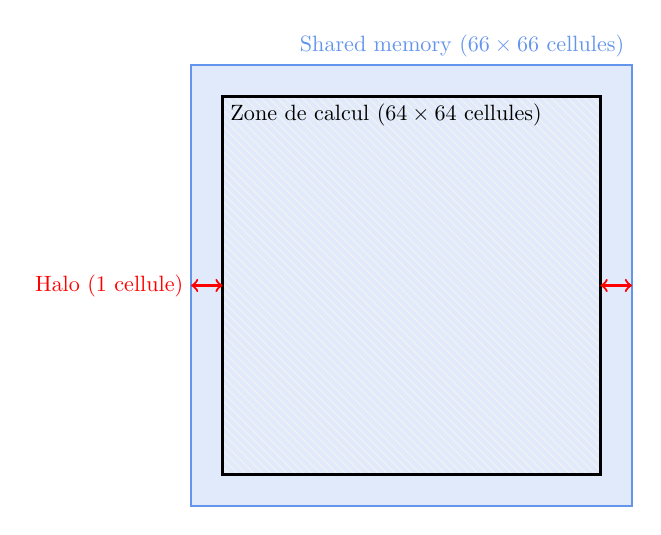
\begin{tikzpicture}[scale=0.8, transform shape]
            % --- Visualisation du Bloc Global (Shared Memory) ---
            % Halo (Shared Memory Size)
            \draw[fill=memblue!20, draw=memblue, thick] (-0.5, -0.5) rectangle (6.5, 6.5);
            \node[memblue, anchor=south east] at (6.5, 6.5) {Shared memory ($66 \times 66$ cellules)};

            % Output Zone (Block Dimensions)
            \draw[fill=white, draw=black, thick, pattern=north west lines, pattern color=gray!10] (0, 0) rectangle (6, 6);
            \node[anchor=north west] at (0, 6) {Zone de calcul ($64 \times 64$ cellules)};

            % Arrows indicating Halo
            \draw[<->, red, thick] (-0.5, 3) -- (0, 3);
            \node[red, left] at (-0.5, 3) {Halo (1 cellule)};
            
            \draw[<->, red, thick] (6, 3) -- (6.5, 3);
        \end{tikzpicture}
    \end{columns}
\end{frame}

% -----------------------------------------------------------------------------
% PARTIE 3: UINT16
% -----------------------------------------------------------------------------
\section{Version Ultime: uint16}

\begin{frame}{Version 3: uint16 (Bit-Packing)}
    \begin{columns}
        \column{0.45\textwidth}
        \textbf{Performance:}
        \begin{itemize}
            \item \textbf{FPS:} \textbf{416.51} ($\times 8.5$ vs naïve)
            \item \textbf{Stratégie:} compression mémoire
        \end{itemize}
        
        \vspace{0.2cm}
        \textbf{Principe:}
        \begin{itemize}
            \item 1 cellule = 1 bit (pas 1 octet)
            \item Grille $32768 \times 32768$ cellules
            \item $\frac{32768 \times 32768}{8 \text{ bits/octet}} = 128 \text{ Mo}$
        \end{itemize}
        
        \column{0.55\textwidth}
        \centering
        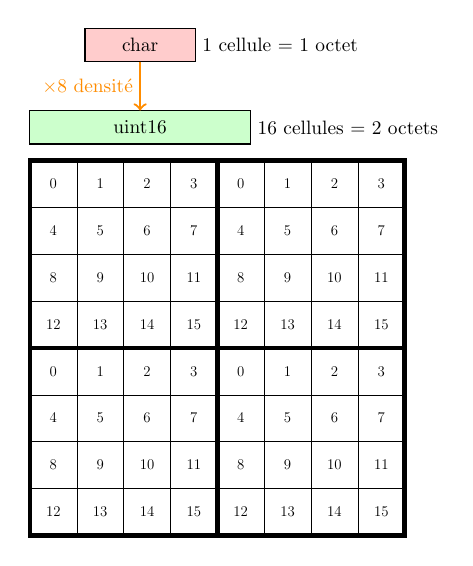
\begin{tikzpicture}[scale=0.7, transform shape]
            % --- Comparison char vs uint16 ---
            \node[draw, fill=red!20, minimum width=2cm, minimum height=0.6cm] (charbox) at (0, 5.5) {char};
            \node[right] at (charbox.east) {1 cellule = 1 octet};
            
            \node[draw, fill=green!20, minimum width=4.0cm, minimum height=0.6cm] (uintbox) at (0, 4) {uint16};
            \node[right] at (uintbox.east) {16 cellules = 2 octets};
            
            \draw[->, thick, coreorange] (charbox.south) -- node[left] {$\times 8$ densité} (uintbox.north);

            % --- 2x2 grid of uint16_t ---
            \begin{scope}[shift={(-2, 0)}, scale=0.85]
                \foreach \BX in {0, 1} {
                    \foreach \BY in {0, 1} {
                        \begin{scope}[shift={(\BX*4, -\BY*4)}]
                            % Border of one uint16
                            \draw[ultra thick, black] (0,0) rectangle (4,4);
                            % Very fine bit separation
                            \draw[ultra thin, black] (0,0) grid (4,4);
                            % Bit indices (0..15)
                            \foreach \r in {0,1,2,3} {
                                \foreach \c in {0,1,2,3} {
                                    \pgfmathtruncatemacro{\idx}{\r*4 + \c}
                                    \node[scale=0.75, font=\large] at (\c+0.5, 3.5-\r) {\idx};
                                }
                            }
                        \end{scope}
                    }
                }
            \end{scope}
        \end{tikzpicture}
    \end{columns}
\end{frame}

\begin{frame}{Architecture du kernel uint16}

    \centering
    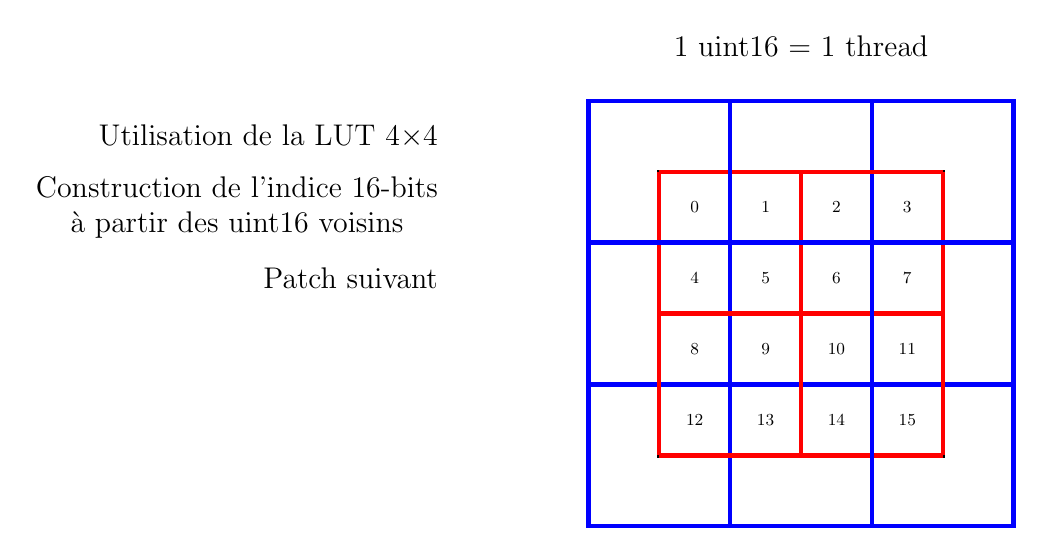
\begin{tikzpicture}[scale=0.9, transform shape]

        % 1. La grille de base (toujours visible)
        \draw[ultra thin, black] (0,0) grid (4,4);
        \foreach \r in {0,1,2,3} {
            \foreach \c in {0,1,2,3} {
                \pgfmathtruncatemacro{\idx}{\r*4 + \c}
                \node[scale=0.75, font=\small] at (\c+0.5, 3.5-\r) {\idx};
            }
        }
        \draw[ultra thick, black] (0,0) rectangle (4,4);
        \node[above, font=\large] at (2,5.5) {1 uint16 = 1 thread};

        % 2. Premier élément (déclenchement au slide 2)
        \pause\node[left, font=\large] at (-3,4.5) {Utilisation de la LUT 4$\times$4};
        % Le red grid est visible sur slide 2, puis disparaît pour laisser place à l'anim, 
        % OU on l'inclus dans l'anim directement (voir ci-dessous)
        \draw<2>[ultra thick, step=2, red] (0,2) grid (2,4);

        % 3. Deuxième élément (déclenchement au slide 3)
        \pause\node[left, font=\large, align=center] at (-3,3.5) {Construction de l'indice 16-bits\\ à partir des uint16 voisins};
        % Étape 1 (Slide 3) : Haut-Gauche
        \draw<3>[ultra thick, step=2, red] (0,2) grid (2,4);
        \draw<3>[ultra thick, step=2, blue] (-1, 1) rectangle (3, 5);
        
        
        \pause\node[left, font=\large, align=center] at (-3,2.5) {Patch suivant};
        % --- ANIMATION (commence au slide 3 et continue) ---
        

        % Étape 2 (Slide 4) : Haut-Droite
        \draw<4>[ultra thick, step=2, red] (2,2) grid (4,4);
        \draw<4>[ultra thick, step=2, blue] (1, 1) rectangle (5, 5);

        % Étape 3 (Slide 5) : Bas-Droite
        \draw<5>[ultra thick, step=2, red] (2,0) grid (4,2);
        \draw<5>[ultra thick, step=2, blue] (1, -1) rectangle (5, 3);

        % Étape 4 (Slide 6) : Bas-Gauche
        \draw<6>[ultra thick, step=2, red] (0,0) grid (2,2);
        \draw<6>[ultra thick, step=2, blue] (-1, -1) rectangle (3, 3);

    \end{tikzpicture}

\end{frame}

\begin{frame}{Architecture du kernel uint16}
    \centering
    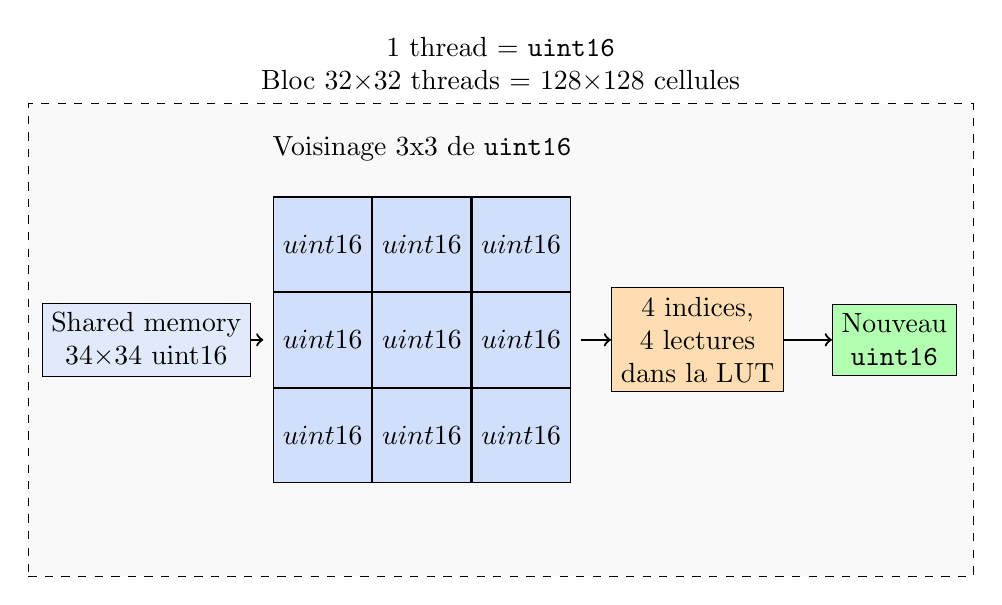
\begin{tikzpicture}[scale=1, transform shape]
        % Main Thread work area
        \node[draw, dashed, fill=gray!5, minimum width=12cm, minimum height=6cm] (gpu) {};
        \node[align=center] at (0, 3.5) {1 thread = \texttt{uint16}\\Bloc 32$\times$32 threads = 128$\times$128 cellules};

        % shared memory area
        \node[draw, fill=memblue!20, align=center] (shared) at (-4.5, 0) {Shared memory\\
        34$\times$34 uint16};
        % \node[above] at (shared.north) {\textbf{Shared Memory} (Halo 66x66 indices)};

        % Inputs in Shared Memory
        \matrix[matrix of math nodes, nodes={draw, minimum size=1.2cm, fill=memblue!30}, ampersand replacement=\&] (shmem) at (-1, 0) {
            uint16 \& uint16 \& uint16 \\
            uint16 \& uint16 \& uint16 \\
            uint16 \& uint16 \& uint16 \\
        };
        \node[above=0.2cm] at (shmem.north) {Voisinage 3x3 de \texttt{uint16}};

        % Bit Magic
        \node[draw, fill=coreorange!30, align=center] (magic) at (2.5,0) {
            4 indices,\\
            4 lectures\\
            dans la LUT
        };
        
        % Output
        \node[draw, fill=green!30, align=center] (res) at (5, 0) {Nouveau\\ \texttt{uint16}};

        % Arrows
        \draw[->, thick] (shared) -- (shmem);
        \draw[->, thick] (shmem) -- (magic);
        \draw[->, thick] (magic) -- (res);
        
    \end{tikzpicture}
\end{frame}


% -----------------------------------------------------------------------------
% CONCLUSION
% -----------------------------------------------------------------------------
\begin{frame}{Résumé des gains de performance}
    \footnotesize
    \centering
    \textbf{Métriques de débit et temps d'exécution} \\
    \vspace{0.1cm}
    \begin{tabular}{lccccc}
        \toprule
        \textbf{Version} & \textbf{Thread/cellule} & \textbf{Durée} (ms) & \textbf{BP Mém.} (Go/s) & \textbf{BP Mém.} (\%) & \textbf{FPS} \\
        \midrule
        \texttt{noif-char}        & 1 & 25.21 & 89.42 & 32.72 & 48.81 \\
        \texttt{lookup4$\times$4} & 4 & 11.21 & 196.02 & 48.30 & 152.04 \\
        \texttt{uint16}           & 16 & \textbf{3.03} & 90.54 & 25.85 & 416.51 \\
        \bottomrule
    \end{tabular}

    \vspace{0.5cm}

    \textbf{Efficacité matérielle} \\
    \vspace{0.1cm}
    \begin{tabular}{lcccc}
        \toprule
        \textbf{Version} & \textbf{Hit L1/TEX} (\%) & \textbf{Occupation Mém.} (\%) & \textbf{SM Busy} (\%) & \textbf{Calcul} (\%) \\
        \midrule
        \texttt{noif-char} & 73.85 & 16.56 & 32.46 & 32.72 \\
        \texttt{lookup4$\times$4} & 72.02 & 31.05 & 46.56 & 48.30 \\
        \texttt{uint16}    & \textbf{95.56} & 20.68 & 39.18 & 37.25 \\
        \bottomrule
    \end{tabular}
\end{frame}


% -----------------------------------------------------------------------------
% ANNEXES : PROFILING
% -----------------------------------------------------------------------------
\begin{frame}{Profiling: noif-char}
    \centering
    \includegraphics[width=0.75\textwidth]{noif-char.png}
\end{frame}

\begin{frame}{Profiling: lookup4$\times$4}
    \centering
    \includegraphics[width=0.75\textwidth]{lookup44.png}
\end{frame}

\begin{frame}{Profiling: uint16 (division par 8 des accès mémoire) }
    \centering
    \includegraphics[width=0.75\textwidth]{uint16.png}
\end{frame}


\end{document}
